\PassOptionsToPackage{unicode=true}{hyperref} % options for packages loaded elsewhere
\PassOptionsToPackage{hyphens}{url}
%
\documentclass[]{book}
\usepackage{lmodern}
\usepackage{amssymb,amsmath}
\usepackage{ifxetex,ifluatex}
\usepackage{fixltx2e} % provides \textsubscript
\ifnum 0\ifxetex 1\fi\ifluatex 1\fi=0 % if pdftex
  \usepackage[T1]{fontenc}
  \usepackage[utf8]{inputenc}
  \usepackage{textcomp} % provides euro and other symbols
\else % if luatex or xelatex
  \usepackage{unicode-math}
  \defaultfontfeatures{Ligatures=TeX,Scale=MatchLowercase}
\fi
% use upquote if available, for straight quotes in verbatim environments
\IfFileExists{upquote.sty}{\usepackage{upquote}}{}
% use microtype if available
\IfFileExists{microtype.sty}{%
\usepackage[]{microtype}
\UseMicrotypeSet[protrusion]{basicmath} % disable protrusion for tt fonts
}{}
\IfFileExists{parskip.sty}{%
\usepackage{parskip}
}{% else
\setlength{\parindent}{0pt}
\setlength{\parskip}{6pt plus 2pt minus 1pt}
}
\usepackage{hyperref}
\hypersetup{
            pdftitle={Guia de Transparência Ativa},
            pdfauthor={Diretoria Central de Transparência Ativa},
            pdfborder={0 0 0},
            breaklinks=true}
\urlstyle{same}  % don't use monospace font for urls
\usepackage{longtable,booktabs}
% Fix footnotes in tables (requires footnote package)
\IfFileExists{footnote.sty}{\usepackage{footnote}\makesavenoteenv{longtable}}{}
\usepackage{graphicx,grffile}
\makeatletter
\def\maxwidth{\ifdim\Gin@nat@width>\linewidth\linewidth\else\Gin@nat@width\fi}
\def\maxheight{\ifdim\Gin@nat@height>\textheight\textheight\else\Gin@nat@height\fi}
\makeatother
% Scale images if necessary, so that they will not overflow the page
% margins by default, and it is still possible to overwrite the defaults
% using explicit options in \includegraphics[width, height, ...]{}
\setkeys{Gin}{width=\maxwidth,height=\maxheight,keepaspectratio}
\setlength{\emergencystretch}{3em}  % prevent overfull lines
\providecommand{\tightlist}{%
  \setlength{\itemsep}{0pt}\setlength{\parskip}{0pt}}
\setcounter{secnumdepth}{5}
% Redefines (sub)paragraphs to behave more like sections
\ifx\paragraph\undefined\else
\let\oldparagraph\paragraph
\renewcommand{\paragraph}[1]{\oldparagraph{#1}\mbox{}}
\fi
\ifx\subparagraph\undefined\else
\let\oldsubparagraph\subparagraph
\renewcommand{\subparagraph}[1]{\oldsubparagraph{#1}\mbox{}}
\fi

% set default figure placement to htbp
\makeatletter
\def\fps@figure{htbp}
\makeatother


\title{Guia de Transparência Ativa}
\author{Diretoria Central de Transparência Ativa}
\date{Última atualização 03/08/2020}

\begin{document}
\maketitle

{
\setcounter{tocdepth}{1}
\tableofcontents
}
\hypertarget{introduuxe7uxe3o}{%
\chapter{INTRODUÇÃO}\label{introduuxe7uxe3o}}

A Lei Federal nº 12.527, de 18 de novembro 2011, conhecida como Lei de Acesso à Informação (LAI), que regula o acesso a informações previsto na Constituição Federal de 1988, estabelece no art. 8º que \textbf{\emph{``É dever dos órgãos e entidades públicas promover, independentemente de requerimentos, a divulgação em local de fácil acesso, no âmbito de suas competências, de informações de interesse coletivo ou geral por eles produzidas ou custodiadas''.}}

No âmbito estadual, a transparência ativa foi regulamentada por meio do Decreto nº 45.969, de 24 de maio de 2012. O capítulo II do Decreto, que é dedicado à transparência ativa, determina a divulgação espontânea (independente de requerimento) de informações de interesse coletivo ou geral, produzidas ou custodiadas pelos órgãos e entidades do Poder Executivo Estadual de Minas Gerais, e define parâmetros a serem adotados no Portal da Transparência do Estado e nos sítios institucionais dos órgãos e entidades.

A Resolução SEPLAG nº 29/2016 estabelece as diretrizes para a estruturação, a elaboração, a manutenção e a administração de sítios eletrônicos de informação de serviços públicos dos órgãos e entidades do Poder Executivo Estadual. No que tange à transparência, ela detalha os requisitos mínimos que devem ser atendidos pelos órgãos e entidades, incluindo a especificação de quais informações devem constar na seção \emph{Transparência} dos sítios institucionais.

A divulgação espontânea do maior número possível de informações, além de facilitar o acesso, também é vantajosa porque tende a reduzir as demandas sobre o assunto nos canais de transparência passiva, minimizando o trabalho e os custos de processamento e gerenciamento dos pedidos de acesso.

Assim, a intenção deste Guia de Transparência Ativa dos sites oficiais do Poder Executivo do Estado de Minas Gerais é auxiliar os órgãos e entidades do Poder Executivo Estadual na implementação do Menu Transparência, conforme previsto no art. 8º, inc. VI do Decreto nº 45.969/2012.

Tendo em vista as exigências previstas nas normas supramencionadas, reforça-se a importância de os órgãos e entidades revisarem e incrementarem o conteúdo da seção/menu \emph{Transparência} de seus sítios eletrônicos.

A Controladoria-Geral do Estado (CGE), por meio da Superintendência Central de Transparência, coloca-se à disposição para esclarecer dúvidas sobre as regras e diretrizes definidas neste guia.

\hypertarget{organizauxe7uxe3o-dos-conteuxfados}{%
\chapter{ORGANIZAÇÃO DOS CONTEÚDOS}\label{organizauxe7uxe3o-dos-conteuxfados}}

A divulgação de dados e informações de forma espontânea relativas à Lei de Acesso à Informação deve ser feita em seção específica/Menu denominada \emph{Transparência}, e disponibilizada na \textbf{página inicial} dos sítios institucionais dos órgãos e entidades.

Os itens a serem divulgados no Menu \textbf{Transparência}, serão divididos em três categorias:

\begin{itemize}
\item
  \textbf{Divulgação obrigatória:} conteúdos que devem constar obrigatoriamente no Menu \textbf{Transparência}, conforme diretrizes da legislação especificada em cada item.
\item
  \textbf{Divulgação específica:} conteúdos a serem disponibilizados no Menu \textbf{Transparência} por determinados órgãos ou entidades quando atendidas as situações especificadas nos itens, conforme diretrizes da legislação específica.
\item
  \textbf{Divulgação opcional:} conteúdos que poderão ser disponibilizados no Menu \textbf{Transparência} a critério do órgão ou entidade.
\end{itemize}

Todos os itens constantes do menu \textbf{Transparência} deverão conter um texto explicativo. As sugestões de textos apresentadas neste guia poderão ser utilizadas pelos órgãos e entidades que assim desejarem.

A nomenclatura e a disposição dos itens de divulgação obrigatória do menu \textbf{Transparência} será padronizada com o objetivo de criar um local único que concentre as informações mínimas e necessárias de transparência ativa de modo a facilitar a localização da informação pelo cidadão e devem observar a seguinte estrutura abaixo:

\begin{itemize}
\tightlist
\item
  \href{servico-informacao.html}{Serviço de Informação ao Cidadão}
\item
  \href{informacoes-classificadas.html}{Informações Classificadas e Desclassificadas}
\item
  \href{programas-acoes.html}{Programas e Ações}
\item
  \href{despesas-receitas.html}{Despesas e Receitas}
\item
  \href{compras-contratos.html}{Compras e Contratos}
\item
  \href{obras-publicas.html}{Obras Públicas}
\item
  \href{convenios-repasses.html}{Convênios, Repasses e Transferências}
\item
  \href{doacoes.html}{Doações e Comodatos}
\item
  \href{servidores.html}{Servidores}
\item
  \href{concursos-publicos.html}{Concursos Públicos}
\item
  \href{dados-abertos.html}{Dados Abertos}
\end{itemize}

Todos os itens de divulgação obrigatória devem ser criados, ainda que não haja conteúdo a ser divulgado. Nesse caso, deve-se criar o item e nele informar, \textbf{de maneira explícita}, que não há, até o momento, conteúdo a ser publicado.

Além dos itens obrigatórios, o órgão e entidade deve disponibilizar, no menu \textbf{Transparência}, outros assuntos estabelecidos em lei que não estão contemplados neste Guia ou que ainda sejam muito demandados pela sociedade ou que sejam considerados de interesse público. Nesses casos, os itens adicionais devem ser inseridos após os obrigatórios e devem conter um texto explicativo relativo ao seu conteúdo.

\begin{itemize}
\tightlist
\item
  Exemplo: \href{https://www.almg.gov.br/consulte/legislacao/completa/completa.html?tipo=LEI\&num=23573\&comp=\&ano=2020}{Lei nº 23.573/2020} que estabelece que o \textbf{Departamento de Trânsito de Minas Gerais -- Detran-MG} divulgará, trimestralmente, \textbf{no seu site}, os valores arrecadados com multas de trânsito, bem como a destinação desses recursos.
\end{itemize}

Como ferramenta de apoio para os órgãos e entidades, apresentamos neste guia para cada item do menu \textbf{Transparência}, os objetivos e os impactos desejados com a criação do item, a legislação de referência, a frequência de atualização do item, quando aplicável, e, o texto padrão contendo a descrição do item que poderá ser utilizado pelo órgão ou entidade que assim o desejar.

Este Guia deve ser utilizado junto com o \textbf{\emph{\href{https://forms.gle/x6rd1aGHzknH8y5m8}{checklist}}} disponibilizado pela Controladoria Geral do Estado, por meio da Subcontroladoria de Transparência e Integridade.

\hypertarget{menu-transparuxeancia}{%
\chapter{MENU TRANSPARÊNCIA}\label{menu-transparuxeancia}}

A divulgação ativa de dados e informações relativas à Lei de Acesso à Informação, nos sítios institucionais dos órgãos ou entidades, deve ser feita em seção específica denominada \textbf{Transparência} e disponibilizada no \textbf{menu principal} das páginas, conforme determina o \href{https://www.almg.gov.br/consulte/legislacao/completa/completa.html?tipo=DEC\&num=45969\&ano=2012}{Decreto Estadual nº 45.969/2012 -- art. 8º, inc. VI}.

O objetivo do menu \textbf{Transparência} é ter um local único e padronizado que concentre as informações mínimas e essenciais dos órgãos e entidades do Poder Executivo Estadual. O menu deve ser composto por um texto explicativo sobre a Lei de Acesso à Informação, por diversos itens e promover o redirecionamento para o Portal da Transparência do Estado de Minas Gerais.

\hypertarget{impactos-esperados}{%
\subsection{Impactos Esperados}\label{impactos-esperados}}

\begin{itemize}
\tightlist
\item
  Padronizar a interface de relacionamento com o cidadão;
\item
  Aumentar a satisfação da sociedade com o fornecimento de informações íntegras e atualizadas;
\item
  Aumentar o controle social.
\end{itemize}

\hypertarget{legislauxe7uxe3o}{%
\subsection{Legislação}\label{legislauxe7uxe3o}}

\begin{itemize}
\tightlist
\item
  \href{https://www.almg.gov.br/consulte/legislacao/completa/completa.html?tipo=DEC\&num=45969\&ano=2012}{Decreto Estadual nº 45.969/2012 -- art. 8º, inc. VI};
\item
  \href{http://www.planejamento.mg.gov.br/sites/default/files/documentos/resolucao_sitios_seplag_29_de_05_07_2016_1.pdf}{Resolução SEPLAG nº 29/2016 -- art. 9º, inc. II, alínea g}.
\end{itemize}

\hypertarget{texto-padruxe3o}{%
\subsection{Texto Padrão}\label{texto-padruxe3o}}

\begin{quote}
Está seção reúne e divulga, de forma espontânea, dados do(a) (NOME DO ÓRGÃO/ENTIDADE) que são de interesse coletivo ou geral com o objetivo de facilitar o acesso à informação pública, conforme determinação da Lei Federal nº 12.527/2011, de 18 de novembro de 2011 e demais legislações que tratam do assunto.

No Menu Transparência estão disponíveis as informações mínimas sobre serviços de informação ao cidadão, informações classificadas e desclassificadas, ações e programas, receitas e despesas, compras e contratos, convênios, repasses e transferências, doações, comodatos e cooperações, pessoal e dados abertos, além de outros tópicos obrigatórios mas específicos para determinados órgãos e entidades e tópicos opcionais, como a participação social.

Para maiores informações sobre a Lei de Acesso à Informação e sua regulamentação no âmbito do Estado de Minas Gerais, acesse o \href{http://www.transparencia.mg.gov.br}{Portal da Transparência}
\end{quote}

\hypertarget{divulgauxe7uxe3o-obrigatuxf3ria}{%
\chapter{DIVULGAÇÃO OBRIGATÓRIA}\label{divulgauxe7uxe3o-obrigatuxf3ria}}

\begin{itemize}
\tightlist
\item
  \href{servico-informacao.html}{Serviço de Informação ao Cidadão}
\item
  \href{informacoes-classificadas.html}{Informações Classificadas e Desclassificadas}
\item
  \href{programas-acoes.html}{Programas e Ações}
\item
  \href{despesas-receitas.html}{Despesas e Receitas}
\item
  \href{compras-contratos.html}{Compras e Contratos}
\item
  \href{obras-publicas.html}{Obras Públicas}
\item
  \href{convenios-repasses.html}{Convênios, Repasses e Transferências}
\item
  \href{doacoes.html}{Doações e Comodatos}
\item
  \href{servidores.html}{Servidores}
\item
  \href{concursos-publicos.html}{Concursos Públicos}
\item
  \href{dados-abertos.html}{Dados Abertos}
\end{itemize}

\hypertarget{serviuxe7o-de-informauxe7uxe3o-ao-cidaduxe3o}{%
\section{Serviço de Informação ao Cidadão}\label{serviuxe7o-de-informauxe7uxe3o-ao-cidaduxe3o}}

\hypertarget{objetivo}{%
\subsection{Objetivo}\label{objetivo}}

\begin{itemize}
\tightlist
\item
  Informar ao cidadão sobre como fazer o pedido de acesso à informação e como obter os relatórios estatísticos com a quantidade de pedidos de acesso à informação do órgão e entidade.
\end{itemize}

\hypertarget{impactos-esperados-1}{%
\subsection{Impactos Esperados}\label{impactos-esperados-1}}

\begin{itemize}
\tightlist
\item
  Organizar e facilitar o procedimento de acesso à informação tanto para o cidadão quanto para a Administração Pública.
\end{itemize}

\hypertarget{legislauxe7uxe3o-1}{%
\subsection{Legislação}\label{legislauxe7uxe3o-1}}

\begin{itemize}
\tightlist
\item
  \href{http://www.planalto.gov.br/ccivil_03/_ato2011-2014/2011/lei/l12527.htm\#art10}{Lei Federal nº 12.527/2011 -- art. 10 a 14};
\item
  \href{http://www.planalto.gov.br/ccivil_03/_ato2011-2014/2012/decreto/d7724.htm}{Decreto Federal nº 7.724/2012 -- art. 9º, 10 e art. 45, inc. III e IV};
\item
  \href{https://www.almg.gov.br/consulte/legislacao/completa/completa.html?tipo=DEC\&num=45969\&ano=2012}{Decreto Estadual nº 45.969/2012 -- art. 12 e 13, art. 46, inc. III e IV};
\item
  \href{http://www.planejamento.mg.gov.br/sites/default/files/documentos/resolucao_sitios_seplag_29_de_05_07_2016_1.pdf}{Resolução SEPLAG nº 29/2016 -- art. 25, inc. V}.
\end{itemize}

\hypertarget{frequuxeancia-de-atualizauxe7uxe3o}{%
\subsection{Frequência de atualização}\label{frequuxeancia-de-atualizauxe7uxe3o}}

\begin{itemize}
\tightlist
\item
  Sempre que houver alteração na legislação do e-SIC.
\item
  Periodicamente, verificar os links de acesso ao e-SIC
\end{itemize}

\hypertarget{texto-padruxe3o-1}{%
\subsection{Texto Padrão}\label{texto-padruxe3o-1}}

\begin{quote}
Nesta seção, são divulgadas informações sobre o Serviço de Informação ao Cidadão (e-SIC), pertinentes ao seu funcionamento, localização e dados de contato no âmbito do(a) (NOME DO ÓRGÃO OU ENTIDADE).

Em Minas Gerais, os pedidos de acesso à informação são feitos por meio do Sistema Eletrônico de Acesso à Informação -- \href{http://www.acessoainformacao.mg.gov.br}{e-SIC}, que permite a solicitação e o acompanhamento dos pedidos e recursos.

As solicitações também podem ser realizadas por meio do telefone 155 (ligação gratuita), ou ainda presencialmente em qualquer \href{http://www.planejamento.mg.gov.br/canais-de-atendimento-ao-cidadao/uais-unidades-de-atendimento-integrado/enderecos-das-uais}{Posto Uai}.

Para acessar aos relatórios estatísticos com a quantidade de pedidos de acesso à informação recebidos, atendidos e indeferidos, assim como informações estatísticas agregadas, consulte os \href{http://www.transparencia.mg.gov.br/o-que-e\#relatórios-gerenciais-–-lei-de-acesso-à-informação}{Relatórios Gerenciais da Lei de Acesso à Informação}.

Responsável pelo monitoramento:
- Nome
- Telefone
- E-mail
\end{quote}

\hypertarget{informauxe7uxf5es-classificadas-e-desclassificadas}{%
\section{Informações classificadas e desclassificadas}\label{informauxe7uxf5es-classificadas-e-desclassificadas}}

\hypertarget{objetivo-1}{%
\subsection{Objetivo}\label{objetivo-1}}

\begin{itemize}
\tightlist
\item
  Informar o rol de informações classificadas em grau de sigilo, bem como o rol de informações desclassificadas nos últimos 12 meses
\end{itemize}

\hypertarget{impactos-esperados-2}{%
\subsection{Impactos Esperados}\label{impactos-esperados-2}}

\begin{itemize}
\tightlist
\item
  Permitir a identificação adequada das informações passíveis de restrições
\item
  Explicitar a frequência de atualização da classificação de informações
\end{itemize}

\hypertarget{legislauxe7uxe3o-2}{%
\subsection{Legislação}\label{legislauxe7uxe3o-2}}

\begin{itemize}
\tightlist
\item
  \href{http://www.planalto.gov.br/ccivil_03/_ato2011-2014/2011/lei/l12527.htm\#art24}{Lei Federal nº 12.527/2011 -- art. 24 e 30};
\item
  \href{http://www.planalto.gov.br/ccivil_03/_ato2011-2014/2012/decreto/d7724.htm\#art45}{Decreto Federal nº 7.724/2012 -- art. 45, inc. I e II};
\item
  \href{https://www.almg.gov.br/consulte/legislacao/completa/completa.html?tipo=DEC\&num=45969\&ano=2012}{Decreto Estadual nº 45.969/2012 -- art 46, inc. I e II};
\item
  \href{http://www.planejamento.mg.gov.br/sites/default/files/documentos/resolucao_sitios_seplag_29_de_05_07_2016_1.pdf}{Resolução SEPLAG nº 29/2016 -- art. 25, inc. VII e art. 26, inc. VIII}.
\end{itemize}

\hypertarget{frequuxeancia-de-atualizauxe7uxe3o-1}{%
\subsection{Frequência de atualização}\label{frequuxeancia-de-atualizauxe7uxe3o-1}}

\begin{itemize}
\tightlist
\item
  Anualmente: em 1º de junho.
\item
  E sempre que houver alteração nas informações classificadas e desclassificadas.
\end{itemize}

\hypertarget{texto-padruxe3o-2}{%
\subsection{Texto Padrão}\label{texto-padruxe3o-2}}

\begin{quote}
Espaço reservado para a divulgação das informações do(a) (NOME DO ÓRGÃO/ENTIDADE) classificadas ou desclassificadas nos graus de sigilo definidos no art. 24 da Lei nº 12.527/2011, em cumprimento ao disposto nos incisos I e II, do art. 45 do Decreto Federal nº 7.724/2012.

Acesse as informações classificadas e desclassificadas do(a) (NOME DO ÓRGÃO OU ENTIDADE), até o dia (informar a última data de atualização)
- Link para documento elaborado pelo órgão ou entidade, conforme orientações da Diretoria Central de Transparência Passiva da Controladoria Geral do Estado.

\begin{itemize}
\tightlist
\item
  Na ausência de informações classificadas ou desclassificadas, o órgão ou entidade deverá informar que no momento não existe conteúdo a ser publicado.
\end{itemize}

O (a) não teve informações classificadas ou desclassificadas nos graus de sigilo reservada, secreta e ultrassecreta, definidos no art. 23 da Lei Federal nº 12.527/11 (Lei de Acesso à Informação), até o dia (informar a última data de atualização)
\end{quote}

\hypertarget{programas-e-auxe7uxf5es}{%
\section{Programas e Ações}\label{programas-e-auxe7uxf5es}}

\hypertarget{objetivo-2}{%
\subsection{Objetivo}\label{objetivo-2}}

\begin{itemize}
\tightlist
\item
  Divulgar todos os instrumentos de planejamento, bem como a relação dos programas e ações do órgão ou entidade, juntamente com informações que permita o seu acompanhamento, conforme orientações do inc. V, §1º, art. 8º da Lei Federal nº12.527/2011.
\end{itemize}

\hypertarget{impactos-esperados-3}{%
\subsection{Impactos Esperados}\label{impactos-esperados-3}}

\begin{itemize}
\tightlist
\item
  Permitir o acompanhamento da execução das metas físicas e financeiras dos programas e ações do órgão ou entidade, por meio da disponibilização das informações referentes e sobre os responsáveis pelos programas e relatórios.
\item
  Informar ao cidadão os instrumentos de planejamento: PPAG, LDO, LOA.
\end{itemize}

\hypertarget{legislauxe7uxe3o-3}{%
\subsection{Legislação}\label{legislauxe7uxe3o-3}}

\begin{itemize}
\tightlist
\item
  \href{http://www.planalto.gov.br/ccivil_03/_ato2011-2014/2011/lei/l12527.htm\#art8}{Lei Federal nº 12.527/2011 -- art. 8, §1º, inc. V};
\item
  \href{http://www.planalto.gov.br/ccivil_03/_ato2011-2014/2012/decreto/d7724.htm}{Decreto Federal nº 7.724/2012 -- art. 7º, §3º, inc. II};
\item
  \href{https://www.almg.gov.br/consulte/legislacao/completa/completa.html?tipo=DEC\&num=45969\&ano=2012}{Decreto Estadual nº 45.969/2012 -- art. 7º, inc. III e art. 8º, inc. VII};
\item
  \href{http://www.planejamento.mg.gov.br/sites/default/files/documentos/resolucao_sitios_seplag_29_de_05_07_2016_1.pdf}{Resolução SEPLAG nº 29/2016 -- art. 25, inc. II e art. 26, inc. II}.
\end{itemize}

\hypertarget{frequuxeancia-de-atualizauxe7uxe3o-2}{%
\subsection{Frequência de atualização}\label{frequuxeancia-de-atualizauxe7uxe3o-2}}

\begin{itemize}
\tightlist
\item
  Anualmente: para a legislação que trata dos instrumentos de planejamento (PPAG, LDO, LOA).
\item
  Bimestralmente: para as informações sobre Ações e Programas -
\item
  Periodicamente, utilizar os links de acesso ao Portal da Transparência da Consulta Programação e Execução do PPAG por Programa.
\end{itemize}

\hypertarget{texto-padruxe3o-3}{%
\subsection{Texto Padrão}\label{texto-padruxe3o-3}}

\begin{quote}
Nesta seção são disponibilizadas as informações dos programas e ações vigentes do(a) (NOME DO ÓRGÃO/ENTIDADE) no ano de XXXX, bem como os instrumentos de planejamento e orçamento do Governo do Estado de Minas Gerais: PPAG, LDO e LOA.

Acesse os dados e informações acerca dos \href{http://www.transparencia.mg.gov.br/planejamento-e-resultados/planejamento-e-monitoramento/programacao-execucao-ppag-programa/ppagprograma-programas/4/2019/0/0}{programas e ações} vigentes no Estado de Minas Gerais, incluindo o do(a) (NOME DO ÓRGÃO/ENTIDADE).

\textbf{Plano Plurianual de Ação Governamental (PPAG):} é o instrumento orientador do planejamento da administração pública de médio prazo. Define qual será o escopo de atuação do Estado para um período de quatro anos, refletido nos programas e ações de governo, com suas respectivas metas físicas e orçamentárias, que serão executados durante esse período.

Acesse o \href{http://transparencia.mg.gov.br/planejamento-e-resultados}{PPAG} na íntegra e os documentos relacionados.

\textbf{Lei de Diretrizes Orçamentárias (LDO):} estabelece quais programas e ações do PPAG serão prioridade, bem como as regras para a elaboração do orçamento e as metas fiscais (projeção da receitas e despesas totais) para os próximos três anos.

Acesse a \href{http://transparencia.mg.gov.br/planejamento-e-resultados}{LDO} na íntegra e os documentos relacionados.

\textbf{Lei Orçamentária Anual (LOA):} detalha os valores (receitas e despesas) definidos para o conjunto de programas e ações do PPAG. Especifica os recursos que irão financiar cada ação e as respectivas despesas.

Acesse a \href{http://transparencia.mg.gov.br/planejamento-e-resultados}{LOA} na íntegra e documentos relacionados.
\end{quote}

\hypertarget{obras-puxfablicas}{%
\section{Obras Públicas}\label{obras-puxfablicas}}

\hypertarget{objetivo-3}{%
\subsection{Objetivo}\label{objetivo-3}}

\begin{itemize}
\tightlist
\item
  Divulgar informações sobre as \textbf{obras públicas cuja execução esteja em andamento}, em cumprimento à Lei Estadual nº 23.386/2019.
\end{itemize}

\hypertarget{impactos-esperados-4}{%
\subsection{Impactos Esperados}\label{impactos-esperados-4}}

\begin{itemize}
\tightlist
\item
  Permitir o acompanhamento por parte do cidadão das obras públicas em andamento, favorecendo a fiscalização da atividade governamental.
\end{itemize}

\hypertarget{legislauxe7uxe3o-4}{%
\subsection{Legislação}\label{legislauxe7uxe3o-4}}

\begin{itemize}
\tightlist
\item
  \href{http://www.planalto.gov.br/ccivil_03/_ato2011-2014/2011/lei/l12527.htm\#art8}{Lei Federal nº 12.527/2011 -- art. 8, §1º, inc. V};
\item
  \href{http://www.planalto.gov.br/ccivil_03/_ato2011-2014/2012/decreto/d7724.htm\#art7}{Decreto Federal nº 7.724/2012 -- art. 7º, §3º, inc. II};
\item
  \href{https://www.almg.gov.br/consulte/legislacao/completa/completa.html?tipo=LEI\&num=23386\&comp=\&ano=2019}{Lei Estadual nº 23.386/2019}.
\end{itemize}

\hypertarget{frequuxeancia-de-atualizauxe7uxe3o-3}{%
\subsection{Frequência de atualização}\label{frequuxeancia-de-atualizauxe7uxe3o-3}}

\begin{itemize}
\tightlist
\item
  Após o início da obra: cópia do contrato e dos termos aditivos, e cópia do projeto básico e do projeto executivo da obra;
\item
  Trimestralmente: relatório de execução da obra, contendo fotografias, cronograma previsto e realizado, medições realizadas e pagamentos autorizados e efetuados.
\end{itemize}

\hypertarget{texto-padruxe3o-4}{%
\subsection{Texto Padrão}\label{texto-padruxe3o-4}}

\begin{quote}
Nesta seção são disponibilizadas as informações sobre as obras públicas em andamento no(a) (NOME DO ÓRGÃO/ENTIDADE).
\end{quote}

\begin{quote}
\begin{longtable}[]{@{}lllllll@{}}
\toprule
\begin{minipage}[b]{0.08\columnwidth}\raggedright
Obra\strut
\end{minipage} & \begin{minipage}[b]{0.10\columnwidth}\raggedright
Objeto\strut
\end{minipage} & \begin{minipage}[b]{0.08\columnwidth}\raggedright
Contrato\strut
\end{minipage} & \begin{minipage}[b]{0.13\columnwidth}\raggedright
Termo Aditivo\strut
\end{minipage} & \begin{minipage}[b]{0.11\columnwidth}\raggedright
Projeto Básico\strut
\end{minipage} & \begin{minipage}[b]{0.14\columnwidth}\raggedright
Projeto Executivo\strut
\end{minipage} & \begin{minipage}[b]{0.17\columnwidth}\raggedright
Relatório Trimestral\strut
\end{minipage}\tabularnewline
\midrule
\endhead
\begin{minipage}[t]{0.08\columnwidth}\raggedright
\strut
\end{minipage} & \begin{minipage}[t]{0.10\columnwidth}\raggedright
\strut
\end{minipage} & \begin{minipage}[t]{0.08\columnwidth}\raggedright
\strut
\end{minipage} & \begin{minipage}[t]{0.13\columnwidth}\raggedright
\strut
\end{minipage} & \begin{minipage}[t]{0.11\columnwidth}\raggedright
\strut
\end{minipage} & \begin{minipage}[t]{0.14\columnwidth}\raggedright
\strut
\end{minipage} & \begin{minipage}[t]{0.17\columnwidth}\raggedright
\strut
\end{minipage}\tabularnewline
\bottomrule
\end{longtable}
\end{quote}

\begin{quote}
Dados da Tabela:
- Obra (nº da obra)
- Objeto (informar o objeto da obra)
- Contrato (número do contrato e link para acesso ao contrato)
- Termo Aditivo (número e link para acesso ao documento)
- Projeto Básico (link para acesso ao documento)
- Projeto Executivo (link para acesso ao documento)
- Relatório Trimestral (número e link para acesso ao relatório)
\end{quote}

\textbf{OBSERVAÇÃO:} Na ausência de Obras Públicas em andamento, o órgão ou entidade deverá informar que no momento não existem obras públicas em andamento.

\begin{quote}
\begin{itemize}
\tightlist
\item
  O(a) (NOME DO ÓRGÃO/ENTIDADE) não possui obras públicas em andamento.
\end{itemize}
\end{quote}

\hypertarget{despesas-e-receitas}{%
\section{Despesas e receitas}\label{despesas-e-receitas}}

\hypertarget{objetivo-4}{%
\subsection{Objetivo}\label{objetivo-4}}

\begin{itemize}
\tightlist
\item
  Disponibilizar informações detalhadas e atualizadas diariamente sobre a execução orçamentária e financeira, bem como sobre suas receitas previstas e arrecadadas.
\end{itemize}

\hypertarget{impactos-esperados-5}{%
\subsection{Impactos Esperados}\label{impactos-esperados-5}}

\begin{itemize}
\tightlist
\item
  Permitir o acompanhamento diário da evolução das receitas e despesas do Estado de Minas Gerais.
\end{itemize}

\hypertarget{legislauxe7uxe3o-5}{%
\subsection{Legislação}\label{legislauxe7uxe3o-5}}

\begin{itemize}
\tightlist
\item
  \href{http://www.planalto.gov.br/ccivil_03/_ato2011-2014/2011/lei/l12527.htm\#art8}{Lei Federal nº 12.527/2011 -- art. 8, §1º, inc. III};
\item
  \href{http://www.planalto.gov.br/ccivil_03/_ato2011-2014/2012/decreto/d7724.htm\#art7}{Decreto Federal nº 7.724/2012 -- art. 7º, §3º, inc. IV};
\item
  \href{https://www.almg.gov.br/consulte/legislacao/completa/completa.html?tipo=DEC\&num=45969\&ano=2012}{Decreto Estadual nº 45.969/2012 -- art. 7º, inc. V};
\item
  \href{http://www.planejamento.mg.gov.br/sites/default/files/documentos/resolucao_sitios_seplag_29_de_05_07_2016_1.pdf}{Resolução SEPLAG nº 29/2016 -- art. 26, inc. III}.
\end{itemize}

\hypertarget{frequuxeancia-de-atualizauxe7uxe3o-4}{%
\subsection{Frequência de atualização}\label{frequuxeancia-de-atualizauxe7uxe3o-4}}

\begin{itemize}
\tightlist
\item
  Periodicamente,utilizar os links de acesso ao Portal da Transparência da Consulta Despesa e da Consulta Receita.
\end{itemize}

\hypertarget{texto-padruxe3o-5}{%
\subsection{Texto Padrão}\label{texto-padruxe3o-5}}

\begin{quote}
Nesta seção são disponibilizadas informações sobre a previsão e arrecadação da receita pública e execução orçamentária e financeira do(a) (NOME DO ÓRGÃO OU ENTIDADE).

\textbf{Despesa pública:} É a aplicação (em dinheiro) de recursos do Estado para custear os serviços de ordem pública ou para investir no próprio desenvolvimento econômico do Estado. É o compromisso de gasto dos recursos públicos, autorizados pelo Poder competente, com o fim de atender a uma necessidade da coletividade prevista no orçamento.

\begin{itemize}
\tightlist
\item
  Acesse as \href{http://www.transparencia.mg.gov.br/despesa-estado/despesa}{despesas públicas estaduais}, incluindo as do(a) (NOME DO ÓRGÃO OU ENTIDADE).
\end{itemize}

\textbf{Receita pública:} Montante em dinheiro recolhido pelo Estado em virtude de arrecadação via impostos, taxas, contribuições e outras fontes de recursos, incorporado ao patrimônio do Estado, que serve para custear as despesas públicas e as necessidades de investimentos públicos.

\begin{itemize}
\tightlist
\item
  Acesse as \href{http://www.transparencia.mg.gov.br/estado-receita}{receitas públicas estaduais}, incluindo as do(a) (NOME DO ÓRGÃO OU ENTIDADE).
\end{itemize}
\end{quote}

\textbf{OBSERVAÇÃO:} Na ausência de receitas arrecadadas pelo próprio órgão/entidade, o órgão ou entidade deverá informar que no momento não existe conteúdo a ser publicado e direcionar para a consulta ``Receita'' do Portal da Transparência.

\hypertarget{compras-e-contratos}{%
\section{Compras e Contratos}\label{compras-e-contratos}}

\hypertarget{objetivo-5}{%
\subsection{Objetivo}\label{objetivo-5}}

\begin{itemize}
\tightlist
\item
  Divulgar informações sobre os processos de compras para aquisição de materiais e serviços nos órgãos e entidades do Estado de Minas Gerais, bem como informações sobre os contratos celebrados entre o Estado e terceiros, incluindo os atos relativos a dispensa ou inexigibilidade de licitação.
\end{itemize}

\hypertarget{impactos-esperados-6}{%
\subsection{Impactos Esperados}\label{impactos-esperados-6}}

\begin{itemize}
\tightlist
\item
  Permitir o acompanhamento da execução dos contratos firmados pela Administração Pública;
\item
  Ampliar a participação da sociedade nos procedimentos licitatórios.
\end{itemize}

\hypertarget{legislauxe7uxe3o-6}{%
\subsection{Legislação}\label{legislauxe7uxe3o-6}}

\begin{itemize}
\tightlist
\item
  \href{http://www.planalto.gov.br/ccivil_03/_ato2011-2014/2011/lei/l12527.htm\#art8}{Lei Federal nº 12.527/2011 -- art. 8, §1º, inc. IV};
\item
  \href{http://www.planalto.gov.br/ccivil_03/_ato2011-2014/2012/decreto/d7724.htm\#art7}{Decreto Federal nº 7.724/2012 -- art. 7º, §3º, inc. V};
\item
  \href{https://www.almg.gov.br/consulte/legislacao/completa/completa.html?tipo=DEC\&num=45969\&ano=2012}{Decreto Estadual nº 45.969/2012 -- art. 7º, inc. VI};
\item
  \href{http://www.planejamento.mg.gov.br/sites/default/files/documentos/resolucao_sitios_seplag_29_de_05_07_2016_1.pdf}{Resolução SEPLAG nº 29/2016 -- art. 25, inc. IV e art. 26, inc. IV};
\item
  \href{https://www.almg.gov.br/consulte/legislacao/completa/completa.html?tipo=LEI\&num=23569\&comp=\&ano=2020}{Lei Estadual nº 23.569/2020 -- art. 1º, inc. I e art. 2º}.
\end{itemize}

\hypertarget{frequuxeancia-de-atualizauxe7uxe3o-5}{%
\subsection{Frequência de atualização}\label{frequuxeancia-de-atualizauxe7uxe3o-5}}

\begin{itemize}
\tightlist
\item
  Procedimento licitatório: em tempo real publicar as fases e toda a documentação pertinente ou disponibilizar link para o Portal de Compras
\item
  Contratos: em tempo real publicar a relação dos contratos vigentes do órgão/entidade, contendo a íntegra do contrato ou utilizar link para a consulta de Compras e Contratos do Portal da Transparência referente a página do processo de compra correspondente.
\item
  Periodicamente, utilizar os links de acesso ao Portal da Transparência e ao Portal de Compras.
\end{itemize}

\hypertarget{texto-padruxe3o-6}{%
\subsection{Texto Padrão}\label{texto-padruxe3o-6}}

\begin{quote}
Nesta seção são disponibilizadas informações relativas aos processos de compras estaduais para aquisição de materiais e serviços, bem como os contratos firmados entre o Estado e terceiros.

\textbf{Compras e Contratos}

Acesse o Portal de Compras para consultar os \href{http://compras.mg.gov.br/}{Procedimentos Licitatórios} em andamento no(a) (NOME DO ÓRGÃO OU ENTIDADE).

Acesse os \href{http://www.transparencia.mg.gov.br/compras-e-patrimonio/compras-e-contratos}{processos de compras} concluído pelo(a) (NOME DO ÓRGÃO OU ENTIDADE).

Consulte e emita o \href{https://www.cagef.mg.gov.br/fornecedor-web/br/gov/prodemge/seplag/fornecedor/publico/index.zul}{Certificado de Regularidade} para Participar de Licitações Públicas no âmbito do Poder Executivo do Estado de Minas Gerais.
\end{quote}

\hypertarget{convuxeanios-repasses-e-transferuxeancias}{%
\section{Convênios, Repasses e Transferências}\label{convuxeanios-repasses-e-transferuxeancias}}

\hypertarget{objetivo-6}{%
\subsection{Objetivo}\label{objetivo-6}}

\begin{itemize}
\tightlist
\item
  Divulgar informações sobre os convênios, repasses e transferências de recursos por meio de convênios de saída, termos de colaboração e fomento, termos de parceria, resoluções e outros instrumentos congêneres;
\item
  Divulgar informações sobre concessões e permissões, nos termos do inc. III, parágrafo único, art. 1º da Lei Estadual nº 23.569/2020.
\end{itemize}

\hypertarget{impactos-esperados-7}{%
\subsection{Impactos Esperados}\label{impactos-esperados-7}}

\begin{itemize}
\tightlist
\item
  Permitir que a sociedade acompanhe os registros de repasses e transferências de recursos financeiros;
\item
  Permitir que a sociedade acompanhe as concessões e permissões firmadas pelo Estado de Minas Gerais.
\end{itemize}

\hypertarget{legislauxe7uxe3o-7}{%
\subsection{Legislação}\label{legislauxe7uxe3o-7}}

\begin{itemize}
\tightlist
\item
  \href{http://www.planalto.gov.br/ccivil_03/_ato2011-2014/2011/lei/l12527.htm\#art8}{Lei Federal nº 12.527/2011 -- art. 8, §1º, inc. II};
\item
  \href{http://www.planalto.gov.br/ccivil_03/_ato2011-2014/2012/decreto/d7724.htm\#art7}{Decreto Federal nº 7.724/2012 -- art. 7º, §3º, inc. III};
\item
  \href{https://www.almg.gov.br/consulte/legislacao/completa/completa.html?tipo=DEC\&num=45969\&ano=2012}{Decreto Estadual nº 45.969/2012 -- art. 7º, inc. IV};
\item
  \href{http://www.planejamento.mg.gov.br/sites/default/files/documentos/resolucao_sitios_seplag_29_de_05_07_2016_1.pdf}{Resolução SEPLAG nº 29/2016 -- art. 25, inc. III e art. 26, inc. V};
\item
  \href{https://www.almg.gov.br/consulte/legislacao/completa/completa.html?tipo=LEI\&num=23569\&comp=\&ano=2020}{Lei Estadual nº 23.569/2020 -- art. 1º, inc. II e III}.
\end{itemize}

\hypertarget{frequuxeancia-de-atualizauxe7uxe3o-6}{%
\subsection{Frequência de atualização}\label{frequuxeancia-de-atualizauxe7uxe3o-6}}

\begin{itemize}
\tightlist
\item
  Periodicamente, utilizar o link de acesso ao Portal da Transparência, para os convênios, repasses e transferências disponíveis na consulta de Convênios/Parcerias de Saída de Recursos.
\item
  Sempre que forem celebrados convênios, repasses e transferências de recursos financeiros que não estejam incluídos na consulta de Convênios/Parcerias de Saída de Recursos do Portal da Transparência.
\item
  Periodicamente, utilizar o link de acesso ao Portal das PPP.
\end{itemize}

\hypertarget{texto-padruxe3o-7}{%
\subsection{Texto Padrão}\label{texto-padruxe3o-7}}

\begin{quote}
Nesta seção são disponibilizadas informações referentes às transferências de recursos públicos realizados pelo Estado por meio de convênios de saída, termos de colaboração e fomento, termos de parceria, resoluções e outros instrumentos congêneres com os órgãos ou entidades públicas ou entidades privadas sem fins lucrativos.

\begin{itemize}
\item
  Acesse os \href{http://www.transparencia.mg.gov.br/convenios/convenios-de-saida}{Convênios de Saída de Recursos} e termos de colaboração e fomento do Estado, incluindo os do(a) (NOME DO ÓRGÃO OU ENTIDADE).
\item
  Acesse os \href{http://www.ppp.mg.gov.br/}{Termos de Concessões -- PPP} realizados por meio de Parcerias Públicos Privadas, incluindo os do(a) (NOME DO ÓRGÃO OU ENTIDADE).
\end{itemize}

Acesse abaixo as transferências de recursos realizadas por meio de resoluções, termos de parceria e outros instrumentos congêneres que não constam na consulta de Convênios/Parcerias de Saída de Recursos do Portal da Transparência e na consulta de PPP:
- O órgão ou entidade deverá disponibilizar o acesso aos documentos de transferências de recursos públicos realizadas pelo Estado, que não estejam disponíveis na consulta de Convênios de Saída do Portal da Transparência.
\end{quote}

\textbf{OBSERVAÇÃO:} Na ausência de convênios e parcerias de saída de recursos, o órgão ou entidade deverá informar que no momento não existe conteúdo para ser publicado e direcionar para a consulta ``Convênios/Parcerias de Saída de Recursos'' do Portal da Transparência.

\hypertarget{servidores}{%
\section{Servidores}\label{servidores}}

\hypertarget{objetivo-7}{%
\subsection{Objetivo}\label{objetivo-7}}

\begin{itemize}
\tightlist
\item
  Divulgar a remuneração e o subsídio recebidos por ocupante de cargo, posto, graduação, função e emprego público, incluindo auxílios, ajudas de custo, jetons e quaisquer outras vantagens pecuniárias, bem como proventos de aposentadoria e pensões daqueles que estiverem na ativa, de maneira individualizada.
\item
  Divulgar as informações sobre os proventos de aposentadoria dos servidores inativos e de pensões pagas pelo Estado de Minas Gerais.
\end{itemize}

\hypertarget{impactos-esperados-8}{%
\subsection{Impactos Esperados}\label{impactos-esperados-8}}

\begin{itemize}
\tightlist
\item
  Permitir o acesso as informações sobre os gastos de pessoal do Estado de Minas Gerais com os servidores ativos, inativos e com pensionistas.
\end{itemize}

\hypertarget{legislauxe7uxe3o-8}{%
\subsection{Legislação}\label{legislauxe7uxe3o-8}}

\begin{itemize}
\tightlist
\item
  \href{http://www.planalto.gov.br/ccivil_03/_ato2011-2014/2012/decreto/d7724.htm\#art7}{Decreto Federal nº 7.724/2012 -- art. 7º, §3º, inc. VI};
\item
  \href{https://www.almg.gov.br/consulte/legislacao/completa/completa.html?tipo=DEC\&num=45969\&ano=2012}{Decreto Estadual nº 45.969/2012 -- art. 4º, inc. VIII};
\item
  \href{http://www.planejamento.mg.gov.br/sites/default/files/documentos/resolucao_sitios_seplag_29_de_05_07_2016_1.pdf}{Resolução SEPLAG nº 29/2016, art. 26, inc. VI}.
\end{itemize}

\hypertarget{frequuxeancia-de-atualizauxe7uxe3o-7}{%
\subsection{Frequência de atualização}\label{frequuxeancia-de-atualizauxe7uxe3o-7}}

\begin{itemize}
\tightlist
\item
  Periodicamente, verificar os links de acesso ao Portal da Transparência da Consulta de Remuneração de Servidores.
\end{itemize}

\hypertarget{texto-padruxe3o-8}{%
\subsection{Texto Padrão}\label{texto-padruxe3o-8}}

\begin{quote}
Nesta seção são disponibilizadas informações sobre os servidores públicos ativos da administração direta, autárquica e fundacional, bem como proventos de aposentadoria e pensões daqueles que estiverem na ativa, de maneira individualizada.

\begin{itemize}
\tightlist
\item
  Acesse a \href{http://www.transparencia.mg.gov.br/estado-pessoal/remuneracao-dos-servidores}{Remuneração dos Servidores Públicos} ativos incluindo os do(a) (NOME DO ÓRGÃO OU ENTIDADE).
\end{itemize}
\end{quote}

\hypertarget{concursos-puxfablicos}{%
\section{Concursos Públicos}\label{concursos-puxfablicos}}

\hypertarget{objetivo-8}{%
\subsection{Objetivo}\label{objetivo-8}}

\begin{itemize}
\tightlist
\item
  Divulgar a íntegra dos editais de concursos públicos para provimentos de cargos e a relação dos aprovados em concurso público.
\end{itemize}

\hypertarget{impactos-esperados-9}{%
\subsection{Impactos Esperados}\label{impactos-esperados-9}}

\begin{itemize}
\tightlist
\item
  Permitir o acompanhamento dos concursos públicos realizados pelo Estado de Minas Gerais e as suas nomeações.
\end{itemize}

\hypertarget{legislauxe7uxe3o-9}{%
\subsection{Legislação}\label{legislauxe7uxe3o-9}}

\begin{itemize}
\tightlist
\item
  \href{http://www.planejamento.mg.gov.br/sites/default/files/documentos/resolucao_sitios_seplag_29_de_05_07_2016_1.pdf}{Resolução SEPLAG nº 29/2016, art. 26, inc. VI conjugado com o anexo IV (Texto Padrão Menu Transparência)}.
\end{itemize}

\hypertarget{frequuxeancia-de-atualizauxe7uxe3o-8}{%
\subsection{Frequência de atualização}\label{frequuxeancia-de-atualizauxe7uxe3o-8}}

\begin{itemize}
\tightlist
\item
  Periodicamente, verificar o link de acesso ao Portal da Transparência da consulta Concursos Realizados;
\item
  Periodicamente, verificar o link de acesso a página da SEPLAG que constam as informações sobre Concursos Públicos.
\end{itemize}

\hypertarget{texto-padruxe3o-9}{%
\subsection{Texto Padrão}\label{texto-padruxe3o-9}}

\begin{quote}
Nesta seção são disponibilizadas também informações sobre os concursos públicos estaduais, incluindo os do(a) (NOME DO ÓRGÃO OU ENTIDADE).

\begin{itemize}
\item
  Acesse os \href{http://www.planejamento.mg.gov.br/concursos-e-estagios/concursos-publicos}{Concursos Públicos em Andamento}, disponíveis na página da Secretaria de Estado de Planejamento e Gestão.
\item
  Acesse os \href{http://www.transparencia.mg.gov.br/estado-pessoal/concursos-realizados}{Concursos Realizados} pelo próprio órgão/entidade.
\end{itemize}
\end{quote}

\textbf{OBSERVAÇÃO:} Na ausência de Concursos Públicos realizados ou em andamento, o órgão ou entidade deverá informar que no momento não existe conteúdo a ser publicado e direcionar para a consulta ``Concursos Realizados'' do Portal da Transparência e/ou ``Concursos Públicos em Andamento'' do sítio da SEPLAG.

\hypertarget{dados-abertos}{%
\section{Dados Abertos}\label{dados-abertos}}

\hypertarget{objetivo-9}{%
\subsection{Objetivo}\label{objetivo-9}}

\begin{itemize}
\tightlist
\item
  Divulgar o maior número de base de dados em formato aberto para que qualquer pessoa possa livremente acessar, utilizar, modificar e compartilhar para qualquer finalidade, estando sujeita, no máximo, à indicação da fonte da base de dados.
\end{itemize}

\hypertarget{impactos-esperados-10}{%
\subsection{Impactos Esperados}\label{impactos-esperados-10}}

\begin{itemize}
\tightlist
\item
  Contribuir para o aumento da transparência do governo, criando melhores possibilidades de controle social das ações
  governamentais.
\item
  Permitir a construção de novas aplicações e conhecimentos pela sociedade.
\end{itemize}

\hypertarget{legislauxe7uxe3o-10}{%
\subsection{Legislação}\label{legislauxe7uxe3o-10}}

\begin{itemize}
\tightlist
\item
  \href{http://www.planalto.gov.br/ccivil_03/_ato2011-2014/2012/decreto/d7724.htm\#art8}{Decreto Federal nº 7.724/2012 -- art. 8º, inc. III e IV};
\item
  \href{https://www.almg.gov.br/consulte/legislacao/completa/completa.html?tipo=DEC\&num=45969\&ano=2012}{Decreto Estadual nº 45.969/2012 -- art. 8º, inc. II e III};
\item
  \href{http://www.planejamento.mg.gov.br/sites/default/files/documentos/resolucao_sitios_seplag_29_de_05_07_2016_1.pdf}{Resolução SEPLAG nº 29/2016 -- art. 25, inc. VIII e art. 26, inc. VII}.
\end{itemize}

\hypertarget{frequuxeancia-de-atualizauxe7uxe3o-9}{%
\subsection{Frequência de atualização}\label{frequuxeancia-de-atualizauxe7uxe3o-9}}

\begin{itemize}
\tightlist
\item
  Periodicamente, utilizar o link de acesso ao Portal de Dados Abertos.
\end{itemize}

\hypertarget{texto-padruxe3o-10}{%
\subsection{Texto Padrão}\label{texto-padruxe3o-10}}

\begin{quote}
Dados abertos governamentais são os dados públicos, produzidos ou sob a tutela do governo, que são disponibilizados ao cidadão em formato bruto e aberto, compreensíveis logicamente, de modo a permitir sua reutilização em aplicações desenvolvidas pela sociedade.

O Estado de Minas Gerais, por meio do \href{http://dados.mg.gov.br/}{Portal de Dados Abertos} disponibiliza a sociedade as bases de dados em formato aberto, os quais podem ser utilizados, modificados e compartilhados.
\end{quote}

\hypertarget{divulgauxe7uxe3o-especuxedfica}{%
\chapter{DIVULGAÇÃO ESPECÍFICA}\label{divulgauxe7uxe3o-especuxedfica}}

\begin{itemize}
\tightlist
\item
  \href{tce.html}{Procedimentos licitatórios enviados para o TCE/MG}
\item
  \href{doacoes.html}{Doações e Comodatos}
\end{itemize}

\hypertarget{procedimentos-licitatuxf3rios-enviados-para-o-tcemg}{%
\section{Procedimentos licitatórios enviados para o TCE/MG}\label{procedimentos-licitatuxf3rios-enviados-para-o-tcemg}}

\hypertarget{objetivo-10}{%
\subsection{Objetivo}\label{objetivo-10}}

\begin{itemize}
\tightlist
\item
  Publicar atos administrativos e documentos relativos a procedimentos licitatórios que deva ser encaminhado ao Tribunal de Contas, por determinação legal ou decisão específica.
\end{itemize}

\hypertarget{impactos-esperados-11}{%
\subsection{Impactos Esperados}\label{impactos-esperados-11}}

\begin{itemize}
\tightlist
\item
  Permitir o acompanhamento pela sociedade dos procedimentos licitatórios enviados ao TCE/MG.
\end{itemize}

\hypertarget{legislauxe7uxe3o-11}{%
\subsection{Legislação}\label{legislauxe7uxe3o-11}}

\begin{itemize}
\tightlist
\item
  \href{https://www.almg.gov.br/consulte/legislacao/completa/completa.html?tipo=LEI\&num=23569\&comp=\&ano=2020}{Lei Estadual nº 23.569/2020 -- art. 1º, caput}.
\end{itemize}

\hypertarget{frequuxeancia-de-atualizauxe7uxe3o-10}{%
\subsection{Frequência de atualização}\label{frequuxeancia-de-atualizauxe7uxe3o-10}}

\begin{itemize}
\tightlist
\item
  Sempre que forem solicitados pelo Tribunal de Contas atos administrativos e documentos relativos a procedimentos licitatórios.
\end{itemize}

\hypertarget{texto-padruxe3o-11}{%
\subsection{Texto Padrão}\label{texto-padruxe3o-11}}

\begin{quote}
Nesta seção são disponibilizadas informações relativas aos atos e procedimentos licitatórios enviados ao Tribunal de Contas do Estado de Minas Gerais, nos termos do art. 1º da Lei Estadual nº 23.569/2020.

\begin{itemize}
\tightlist
\item
  Procedimento Licitatório X (informar o tipo de procedimento licitatório e número)

  \begin{itemize}
  \tightlist
  \item
    Lista dos documentos encaminhados, com link para acesso ou pdf do documento.
  \end{itemize}
\end{itemize}
\end{quote}

\hypertarget{doauxe7uxf5es-e-comodatos}{%
\section{Doações e Comodatos}\label{doauxe7uxf5es-e-comodatos}}

\hypertarget{objetivo-11}{%
\subsection{Objetivo}\label{objetivo-11}}

\begin{itemize}
\tightlist
\item
  Publicar doações e comodatos celebrados, contendo informações sobre: nome do doador ou comodante; CNPJ ou CPF do doador ou comodante; ojbeto da doação ou comodato e, quando for o caso, seu quantitativo; a vigência do comodato; o valor estimado do bem ou serviço doado ou oferecido em comodato..
\end{itemize}

\hypertarget{impactos-esperados-12}{%
\subsection{Impactos Esperados}\label{impactos-esperados-12}}

\begin{itemize}
\tightlist
\item
  Permitir que a sociedade acompanhe as doações de bens e serviços ao Estado de Minas Gerais.
\item
  Falicitar a localização dos registros de doações de bens e serviços.
\end{itemize}

\hypertarget{legislauxe7uxe3o-12}{%
\subsection{Legislação}\label{legislauxe7uxe3o-12}}

\begin{itemize}
\tightlist
\item
  \href{https://www.almg.gov.br/consulte/legislacao/completa/completa.html?tipo=DEC\&num=47611\&comp=\&ano=2019}{Decreto Estadual nº 47.611/2019 - art. 17 e 18}.
\end{itemize}

\hypertarget{frequuxeancia-de-atualizauxe7uxe3o-11}{%
\subsection{Frequência de atualização}\label{frequuxeancia-de-atualizauxe7uxe3o-11}}

\begin{itemize}
\tightlist
\item
  Após a formalização do ato, divulgar no próprio sítio eletrônico a relação das doações ou comodatos recebidos pelos órgãos/entidades, contendo o nome do doador ou comodante; o CNPJ ou CPF do doador ou comodante; o objeto da doação ou comodato e, quando for o caso, seu quantitativo; a vigência do comodato; o valor estimado do bem ou serviço doado ou oferecido em comodato;
\item
  Após a formalização do ato, enviar planilha em formato CSV para o e-mail \href{mailto:transparencia@cge.mg.gov.br}{\nolinkurl{transparencia@cge.mg.gov.br}}, da Superintendência Central de Transparência para publicação em formato aberto, contendo o nome do doador ou comodante; o CNPJ ou CPF do doador ou comodante; o objeto da doação ou comodato e, quando for o caso, seu quantitativo; a vigência do comodato; o valor estimado do bem ou serviço doado ou oferecido em comodato.
\end{itemize}

\hypertarget{texto-padruxe3o-12}{%
\subsection{Texto Padrão}\label{texto-padruxe3o-12}}

\begin{quote}
Nesta seção são disponibilizadas a relação das doações e comodatos para o Governo de Minas Gerais, em consonância com o art. 18 do Decreto nº 47.611/2019.

\begin{itemize}
\tightlist
\item
  Acesse aqui a relação das doações e comodatos para o Governo de Minas Gerais, por meio do(a) (NOME DO ÓRGÃO OU ENTIDADE).
\end{itemize}
\end{quote}

\begin{itemize}
\tightlist
\item
  Incluir no documento as seguintes informações:

  \begin{itemize}
  \tightlist
  \item
    nome do doador ou comodante;
  \item
    CNPJ ou CPF do doador ou comodante;
  \item
    objeto da doação ou comodato e, quando for o caso, seu quantitativo;
  \item
    vigência do comodato;
  \item
    valor estimado do bem ou serviço doado ou oferecido em comodato.
  \end{itemize}
\end{itemize}

\hypertarget{divulgauxe7uxe3o-opcional}{%
\chapter{DIVULGAÇÃO OPCIONAL}\label{divulgauxe7uxe3o-opcional}}

\begin{itemize}
\tightlist
\item
  \href{participacao-social.html}{Participação Social}
\item
  \href{convenios-entrada.html}{Convênios de Entrada}
\item
  \href{bens.html}{Bens}
\end{itemize}

\hypertarget{participauxe7uxe3o-social}{%
\section{Participação Social}\label{participauxe7uxe3o-social}}

\hypertarget{objetivo-12}{%
\subsection{Objetivo}\label{objetivo-12}}

\begin{itemize}
\tightlist
\item
  Criar um local único e padronizado que concentre as informações sobre participação social.
\end{itemize}

\hypertarget{impactos-esperados-13}{%
\subsection{Impactos Esperados}\label{impactos-esperados-13}}

\begin{itemize}
\tightlist
\item
  Fomentar o diálogo com a população e promover a participação social.
\item
  Permitir a participação da sociedade na construção de políticas públicas.
\end{itemize}

\hypertarget{legislauxe7uxe3o-13}{%
\subsection{Legislação}\label{legislauxe7uxe3o-13}}

\begin{itemize}
\tightlist
\item
  \href{http://www.planalto.gov.br/ccivil_03/_ato2011-2014/2011/lei/l12527.htm\#art9}{Lei Federal nº 12.527/2011 -- art. 9º, inc. II};
\item
  \href{https://www.almg.gov.br/consulte/legislacao/completa/completa.html?tipo=DEC\&num=45969\&ano=2012}{Decreto Estadual nº 45.969/2012 -- art. 14, §6º}.
\end{itemize}

\hypertarget{frequuxeancia-de-atualizauxe7uxe3o-12}{%
\subsection{Frequência de atualização}\label{frequuxeancia-de-atualizauxe7uxe3o-12}}

\begin{itemize}
\tightlist
\item
  Periodicamente, sempre que surgirem novas informações sobre participação social.
\end{itemize}

\hypertarget{texto-padruxe3o-13}{%
\subsection{Texto Padrão}\label{texto-padruxe3o-13}}

\begin{quote}
Conheça os espaços existentes e as atividades desenvolvidas pelo(a) (NOME DO ÓRGÃO OU ENTIDADE) para fomentar o diálogo com a população e a participação social na construção das políticas públicas.

Tópicos que podem ser incluídos nessa seção, de acordo com as especificidades de cada órgão/entidade:

\begin{itemize}
\tightlist
\item
  Conselhos e Órgãos Colegiados
\item
  Conferências
\item
  Audências Públicas
\item
  Consultas Públicas
\item
  Fundos Vinculados
\item
  Ações de promoção da Cidadania
\end{itemize}

Conheça os demais Conselhos de Políticas Públicas do Estado de Minas Gerais. Acesse o \href{http://portaldosconselhos.cge.mg.gov.br/}{Portal dos Conselhos} e faça parte da construção de políticas públicas de seu interesse!
\end{quote}

\hypertarget{convuxeanios-de-entrada}{%
\section{Convênios de Entrada}\label{convuxeanios-de-entrada}}

\hypertarget{objetivo-13}{%
\subsection{Objetivo}\label{objetivo-13}}

\begin{itemize}
\tightlist
\item
  Criar um local único e padronizado que concentre as informações sobre os recursos recebidos pelo órgão ou entidade.
\end{itemize}

\hypertarget{impactos-esperados-14}{%
\subsection{Impactos Esperados}\label{impactos-esperados-14}}

\begin{itemize}
\tightlist
\item
  Permitir que a sociedade acompanhe as informações de convênios de entrada de recursos celebrados pelo Estado.
\end{itemize}

\hypertarget{legislauxe7uxe3o-14}{%
\subsection{Legislação}\label{legislauxe7uxe3o-14}}

\begin{itemize}
\tightlist
\item
  \href{http://www.planalto.gov.br/ccivil_03/_ato2011-2014/2011/lei/l12527.htm}{Lei Federal nº 12.527/2011}.
\end{itemize}

\hypertarget{frequuxeancia-de-atualizauxe7uxe3o-13}{%
\subsection{Frequência de atualização}\label{frequuxeancia-de-atualizauxe7uxe3o-13}}

\begin{itemize}
\tightlist
\item
  Periodicamente, utilizar o link de acesso ao Portal da Transparência a consulta de Convênios de Entrada.
\item
  Sempre que forem celebrados convênios de entrada de recursos que não estejam incluídos na consulta Convênios de Entrada do Portal da Transparência
\end{itemize}

\hypertarget{texto-padruxe3o-14}{%
\subsection{Texto Padrão}\label{texto-padruxe3o-14}}

\begin{quote}
Nesta seção são disponibilizadas informações referentes à transferência de recursos públicos para os órgão e entidades do Estado de Minas Gerais por meio de convênios de entrada.

\begin{itemize}
\item
  Acesse os \href{http://www.transparencia.mg.gov.br/convenios/convenio-entrada}{Convênios de Entrada}, incluindo os do(a) (NOME DO ÓRGÃO OU ENTIDADE).
\item
  Acesse os convênios de entrada que não constam na consulta de Convênios de Entrada do Portal da Transparência:

  O órgão ou entidade deverá disponibilizar o acesso aos documentos dos convênios de entrada de recursos que não estejam disponíveis na consulta de Convênios de Entrada do Portal da Transparência.
\end{itemize}
\end{quote}

\hypertarget{bens}{%
\section{Bens}\label{bens}}

\hypertarget{objetivo-14}{%
\subsection{Objetivo}\label{objetivo-14}}

\begin{itemize}
\tightlist
\item
  Criar um local único e padronizado que concentre as informações sobre o patrimônio mobiliário e sobre a frota ativa do Estado de Minas Gerais.
\end{itemize}

\hypertarget{impactos-esperados-15}{%
\subsection{Impactos Esperados}\label{impactos-esperados-15}}

\begin{itemize}
\tightlist
\item
  Permitir que a sociedade acompanhe a utilização e a destinação dos bens estaduais.
\end{itemize}

\hypertarget{legislauxe7uxe3o-15}{%
\subsection{Legislação}\label{legislauxe7uxe3o-15}}

\begin{itemize}
\tightlist
\item
  \href{http://www.planalto.gov.br/ccivil_03/_ato2011-2014/2011/lei/l12527.htm}{Lei Federal nº 12.527/2011}.
\end{itemize}

\hypertarget{frequuxeancia-de-atualizauxe7uxe3o-14}{%
\subsection{Frequência de atualização}\label{frequuxeancia-de-atualizauxe7uxe3o-14}}

\begin{itemize}
\tightlist
\item
  Periodicamente, utilizar os links do Portal da Transparência das consultas de Patrimônio e Gestão de Frota.
\end{itemize}

\hypertarget{texto-padruxe3o-15}{%
\subsection{Texto Padrão}\label{texto-padruxe3o-15}}

\begin{quote}
Nesta seção são disponibilizados dados da frota de veículos terrestres ativa que estão a serviço do Estado, incluindo informações sobre a manutenções e abastecimentos desses veículos e também informações sobre o patrimônio mobiliário do Estado, incluindo os bens que se encontram em uso ou não, podendo as consultas serem realizadas por órgão ou entidade.

\begin{itemize}
\item
  Acesse a listagem dos \href{http://www.transparencia.mg.gov.br/compras-e-patrimonio/patrimonio}{Bens Móveis} do Estado de Minas Gerais.
\item
  Acesse a \href{http://www.transparencia.mg.gov.br/compras-e-patrimonio/gestao-de-frota}{Frota} do Estado de Minas Gerais.
\end{itemize}
\end{quote}

\hypertarget{dispositivos-legais}{%
\chapter{DISPOSITIVOS LEGAIS}\label{dispositivos-legais}}

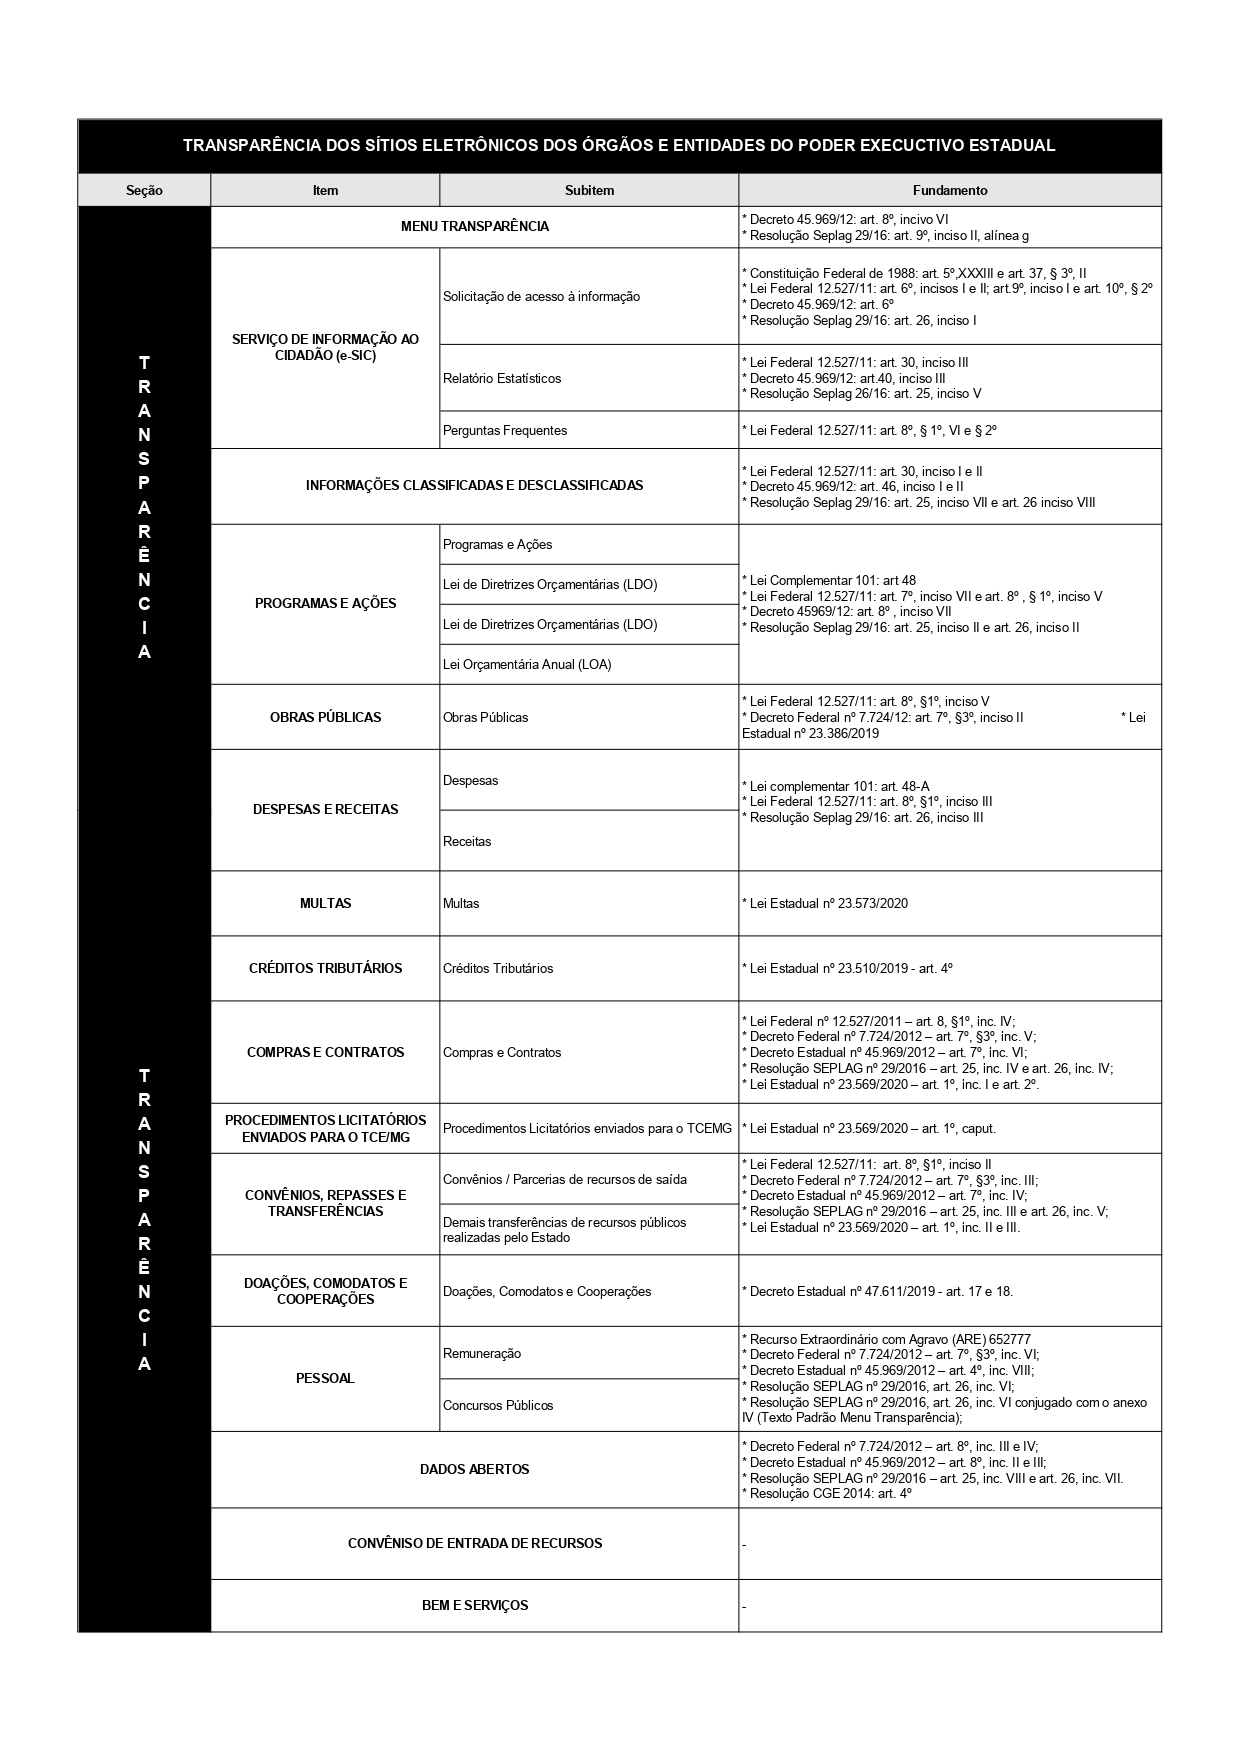
\includegraphics{static/quadro_guia_atualizado.jpg}

\hypertarget{aspectos-tecnoluxf3gicos}{%
\chapter{ASPECTOS TECNOLÓGICOS}\label{aspectos-tecnoluxf3gicos}}

Os órgãos e entidades deverão observar os requisitos mínimos para disponibilização das informações nos sítios institucionais, conforme determina o \href{http://www.planalto.gov.br/ccivil_03/_ato2011-2014/2011/lei/l12527.htm\#art8\%C2\%A73}{art. 8º da Lei Federal nº 12.527/2011}:

\begin{itemize}
\item
  Ferramentas de pesquisa de conteúdo: o sitio institucional deverá possuir ferramenta de pesquisa por palavra em todo o conteúdo;
\item
  Gravação de relatórios em diversos formatos eletrônicos, inclusive abertos e não proprietários: os dados deverão estar disponíveis para download em formatos abertos e não proprietários, tais como planilhas e textos, de modo a facilitar a análise de informações;
\item
  Acesso automatizado por sistemas externos: possibilitar que os dados sejam acessados de forma automatizada por sistemas externos, em formatos abertos, estruturados e legíveis por máquina. Exemplo: Os dados disponíveis deverão ser acessados por sistemas externos sem qualquer tipo de intervenção humana direta, tais como a utilização de API;
\item
  Indicar local e instruções que permitam ao interessado comunicar-se, por via eletrônica ou telefônica, como o órgão ou entidade detentora do sítio; e
\item
  Acessibilidade ao conteúdo para pessoas com deficiência: adotar as medidas necessárias para garantir a acessibilidade de conteúdo para pessoas com deficiência. Exemplo: O menu principal deverá estar no topo da página, ser acessível por meio de teclado e sem a necessidade de rolagem de página.
\end{itemize}

\hypertarget{checklist}{%
\chapter{CHECKLIST}\label{checklist}}

\hypertarget{avaliauxe7uxe3o-da-transparuxeancia-ativa-dos-uxf3rguxe3os-e-entidades}{%
\subsection*{AVALIAÇÃO DA TRANSPARÊNCIA ATIVA DOS ÓRGÃOS E ENTIDADES}\label{avaliauxe7uxe3o-da-transparuxeancia-ativa-dos-uxf3rguxe3os-e-entidades}}
\addcontentsline{toc}{subsection}{AVALIAÇÃO DA TRANSPARÊNCIA ATIVA DOS ÓRGÃOS E ENTIDADES}

\textbf{IMPORTANTE:} A avaliação do sítio eletrônico deve ser iniciada e finalizada no mesmo dia

\begin{itemize}
\tightlist
\item
  DATA DE APLICAÇÃO DO CHECKLIST
\item
  ENDEREÇO DE E-MAIL INSTITUCIONAL
\item
  NOME DO(A) CONTROLADOR(A)
\item
  SIGLA DO ÓRGÃO/ENTIDADE
\item
  O ÓRGÃO/ENTIDADE TEM SÍTIO INSTITUCIONAL

  \begin{itemize}
  \tightlist
  \item
    {[} {]} SIM
  \item
    {[} {]} NÃO
  \end{itemize}
\end{itemize}

\hypertarget{menu-transparuxeancia-1}{%
\subsubsection*{MENU TRANSPARÊNCIA}\label{menu-transparuxeancia-1}}
\addcontentsline{toc}{subsubsection}{MENU TRANSPARÊNCIA}

\begin{itemize}
\tightlist
\item
  O Menu \textbf{Transparência} esta disponível na página principal do sítio eletrônico do órgão ou entidade?

  \begin{itemize}
  \tightlist
  \item
    {[} {]} ATENDE TOTALMENTE
  \item
    {[} {]} NÃO ATENDE
  \end{itemize}
\item
  O link do Menu \textbf{Transparência} está funcionando corretamente?

  \begin{itemize}
  \tightlist
  \item
    {[} {]} ATENDE TOTALMENTE
  \item
    {[} {]} NÃO ATENDE
  \end{itemize}
\item
  No Menu \textbf{Transparência} tem o texto padrão sobre o Menu Transparência?

  \begin{itemize}
  \tightlist
  \item
    {[} {]} ATENDE TOTALMENTE
  \item
    {[} {]} NÃO ATENDE
  \end{itemize}
\end{itemize}

\hypertarget{serviuxe7o-de-informauxe7uxe3o-ao-cidaduxe3o-1}{%
\subsubsection*{SERVIÇO DE INFORMAÇÃO AO CIDADÃO}\label{serviuxe7o-de-informauxe7uxe3o-ao-cidaduxe3o-1}}
\addcontentsline{toc}{subsubsection}{SERVIÇO DE INFORMAÇÃO AO CIDADÃO}

\begin{itemize}
\tightlist
\item
  No menu ``Transparência'' tem o Item ``Serviço de Informação ao Cidadão''?

  \begin{itemize}
  \tightlist
  \item
    {[} {]} ATENDE TOTALMENTE
  \item
    {[} {]} NÃO ATENDE
  \end{itemize}
\item
  Dentro do Item ``Serviço de Informação ao Cidadão'': tem o texto explicativo sobre a LAI

  \begin{itemize}
  \tightlist
  \item
    {[} {]} ATENDE TOTALMENTE
  \item
    {[} {]} NÃO ATENDE
  \end{itemize}
\item
  Dentro do Item ``Serviço de Informação ao Cidadão'': tem o link para realizar solicitação de acesso à informação (e-SIC), direcionando corretamente para a página do e-SIC do Portal da Transparência

  \begin{itemize}
  \tightlist
  \item
    {[} {]} ATENDE TOTALMENTE
  \item
    {[} {]} NÃO ATENDE
  \end{itemize}
\item
  Dentro do Item ``Serviço de Informação ao Cidadão'': tem o link para acessar os relatórios dos pedidos de acesso à informação, direcionando corretamente para a página dos relatórios dos pedidos do Portal da Transparência.

  \begin{itemize}
  \tightlist
  \item
    {[} {]} ATENDE TOTALMENTE
  \item
    {[} {]} NÃO ATENDE
  \end{itemize}
\item
  Dentro do Item ``Serviço de Informação ao Cidadão'': tem informações sobre o responsável pelo e-SIC no órgão/entidade, com dados de nome, telefone e e-mail para contato?

  \begin{itemize}
  \tightlist
  \item
    {[} {]} ATENDE TOTALMENTE
  \item
    {[} {]} NÃO ATENDE
  \end{itemize}
\end{itemize}

\hypertarget{informauxe7uxf5es-classificadas-e-desclassificadas-1}{%
\subsubsection*{INFORMAÇÕES CLASSIFICADAS E DESCLASSIFICADAS}\label{informauxe7uxf5es-classificadas-e-desclassificadas-1}}
\addcontentsline{toc}{subsubsection}{INFORMAÇÕES CLASSIFICADAS E DESCLASSIFICADAS}

\begin{itemize}
\tightlist
\item
  No menu ``Transparência'': tem o item ``Informações Classificadas e Desclassificadas''

  \begin{itemize}
  \tightlist
  \item
    {[} {]} ATENDE TOTALMENTE
  \item
    {[} {]} NÃO ATENDE
  \end{itemize}
\item
  Dentro do item ``Informações Classificadas e Desclassificadas'': tem o texto explicativo sobre classificação e desclassificação de informações

  \begin{itemize}
  \tightlist
  \item
    {[} {]} ATENDE TOTALMENTE
  \item
    {[} {]} NÃO ATENDE
  \end{itemize}
\end{itemize}

\hypertarget{informauxe7uxf5es-classificadas-e-desclassificadas---para-uxf3rguxe3os-que-possuem-informauxe7uxf5es-classificadas-e-desclassificadas}{%
\subsubsection*{INFORMAÇÕES CLASSIFICADAS E DESCLASSIFICADAS - para órgãos que POSSUEM informações Classificadas e Desclassificadas}\label{informauxe7uxf5es-classificadas-e-desclassificadas---para-uxf3rguxe3os-que-possuem-informauxe7uxf5es-classificadas-e-desclassificadas}}
\addcontentsline{toc}{subsubsection}{INFORMAÇÕES CLASSIFICADAS E DESCLASSIFICADAS - para órgãos que POSSUEM informações Classificadas e Desclassificadas}

\begin{itemize}
\tightlist
\item
  Dentro do item ``Informações Classificadas e Desclassificadas'': tem o link para documento contendo as informações classificadas e desclassificadas

  \begin{itemize}
  \tightlist
  \item
    {[} {]} ATENDE TOTALMENTE
  \item
    {[} {]} NÃO ATENDE
  \item
    {[} {]} NÃO SE APLICA
  \end{itemize}
\item
  Dentro do item ``Informações Classificadas e Desclassificadas'': consta a data da última atualização das informações classificadas e desclassificadas

  \begin{itemize}
  \tightlist
  \item
    {[} {]} ATENDE TOTALMENTE
  \item
    {[} {]} NÃO ATENDE
  \item
    {[} {]} NÃO SE APLICA
  \end{itemize}
\end{itemize}

\hypertarget{informauxe7uxf5es-classificadas-e-desclassificadas---para-uxf3rguxe3os-que-nuxe3o-possuem-informauxe7uxf5es-classificadas-e-desclassificadas}{%
\subsubsection*{INFORMAÇÕES CLASSIFICADAS E DESCLASSIFICADAS - para órgãos que NÃO POSSUEM informações Classificadas e Desclassificadas}\label{informauxe7uxf5es-classificadas-e-desclassificadas---para-uxf3rguxe3os-que-nuxe3o-possuem-informauxe7uxf5es-classificadas-e-desclassificadas}}
\addcontentsline{toc}{subsubsection}{INFORMAÇÕES CLASSIFICADAS E DESCLASSIFICADAS - para órgãos que NÃO POSSUEM informações Classificadas e Desclassificadas}

\begin{itemize}
\tightlist
\item
  Dentro do item ``Informações Classificadas e Desclassificadas'': foi colocado texto explicativo padrão.

  \begin{itemize}
  \tightlist
  \item
    {[} {]} ATENDE TOTALMENTE
  \item
    {[} {]} NÃO ATENDE
  \item
    {[} {]} NÃO SE APLICA
  \end{itemize}
\item
  Dentro do item ``Informações Classificadas e Desclassificadas'': consta a data da última atualização das informações classificadas e desclassificadas

  \begin{itemize}
  \tightlist
  \item
    {[} {]} ATENDE TOTALMENTE
  \item
    {[} {]} NÃO ATENDE
  \item
    {[} {]} NÃO SE APLICA
  \end{itemize}
\end{itemize}

\hypertarget{programas-e-auxe7uxf5es-1}{%
\subsubsection*{PROGRAMAS E AÇÕES}\label{programas-e-auxe7uxf5es-1}}
\addcontentsline{toc}{subsubsection}{PROGRAMAS E AÇÕES}

\begin{itemize}
\tightlist
\item
  Dentro do menu ``Transparência'' tem o item ``Programas e Ações''

  \begin{itemize}
  \tightlist
  \item
    {[} {]} ATENDE TOTALMENTE
  \item
    {[} {]} NÃO ATENDE
  \end{itemize}
\item
  Dentro do item ``Programas e Ações'': tem o link para a página da consulta de Programação e Execução do PPAG por programa do Portal da Transparência

  \begin{itemize}
  \tightlist
  \item
    {[} {]} ATENDE TOTALMENTE
  \item
    {[} {]} NÃO ATENDE
  \end{itemize}
\item
  Dentro do item ``Programas e Ações'': tem o documento do PPAG ou link correto para a página da SEPLAG

  \begin{itemize}
  \tightlist
  \item
    {[} {]} ATENDE TOTALMENTE
  \item
    {[} {]} NÃO ATENDE
  \end{itemize}
\item
  Dentro do item ``Programas e Ações'': tem o documento da LDO ou link correto para a página da SEPLAG

  \begin{itemize}
  \tightlist
  \item
    {[} {]} ATENDE TOTALMENTE
  \item
    {[} {]} NÃO ATENDE
  \end{itemize}
\item
  Dentro do item ``Programas e Ações'': tem o documento da LOA ou link correto para a página da SEPLAG

  \begin{itemize}
  \tightlist
  \item
    {[} {]} ATENDE TOTALMENTE
  \item
    {[} {]} NÃO ATENDE
  \end{itemize}
\end{itemize}

\hypertarget{obras-puxfablicas-1}{%
\subsubsection*{OBRAS PÚBLICAS}\label{obras-puxfablicas-1}}
\addcontentsline{toc}{subsubsection}{OBRAS PÚBLICAS}

\begin{itemize}
\tightlist
\item
  Dentro do menu ``Transparência'' tem o item ``Obras Públicas''

  \begin{itemize}
  \tightlist
  \item
    {[} {]} ATENDE TOTALMENTE
  \item
    {[} {]} NÃO ATENDE
  \end{itemize}
\item
  Para órgãos/entidades que possuem obras em andamento: Dentro do item ``Obras Públicas'': tem informações sobre as obras públicas em andamento no órgão ou entidade, como: objeto, contrato, termo aditivo, projeto básico, projeto executivo e relatório trimestral para os órgãos/entidades que possuem obras em andamento

  \begin{itemize}
  \tightlist
  \item
    {[} {]} ATENDE TOTALMENTE
  \item
    {[} {]} NÃO ATENDE
  \item
    {[} {]} NÃO SE APLICA
  \end{itemize}
\item
  Para órgãos e entidades que não possuem obras em andamento: Dentro do item ``Obras Públicas'': tem a informação de que não existirem obras em andamento para órgãos/entidades que não possuem obras em andamento.

  \begin{itemize}
  \tightlist
  \item
    {[} {]} ATENDE TOTALMENTE
  \item
    {[} {]} NÃO ATENDE
  \item
    {[} {]} NÃO SE APLICA
  \end{itemize}
\end{itemize}

\hypertarget{despesas-e-receitas-1}{%
\subsubsection*{DESPESAS E RECEITAS}\label{despesas-e-receitas-1}}
\addcontentsline{toc}{subsubsection}{DESPESAS E RECEITAS}

\begin{itemize}
\tightlist
\item
  Dentro do menu ``Transparência'' tem o item ``Despesas e Receitas''

  \begin{itemize}
  \tightlist
  \item
    {[} {]} ATENDE TOTALMENTE
  \item
    {[} {]} NÃO ATENDE
  \end{itemize}
\item
  Dentro do item ``Despesas e Receitas'': tem o texto explicativo sobre Despesas

  \begin{itemize}
  \tightlist
  \item
    {[} {]} ATENDE TOTALMENTE
  \item
    {[} {]} NÃO ATENDE
  \end{itemize}
\item
  Dentro do item ``Despesas e Receitas'': tem o link direcionando corretamente para a consulta de Despesa do Portal da Transparência

  \begin{itemize}
  \tightlist
  \item
    {[} {]} ATENDE TOTALMENTE
  \item
    {[} {]} NÃO ATENDE
  \end{itemize}
\item
  Dentro do item ``Despesas e Receitas'': tem o texto explicativo sobre Receitas

  \begin{itemize}
  \tightlist
  \item
    {[} {]} ATENDE TOTALMENTE
  \item
    {[} {]} NÃO ATENDE
  \end{itemize}
\item
  Dentro do item ``Despesas e Receitas'': tem o link direcionando corretamente para a consulta de Receita do Portal da Transparência

  \begin{itemize}
  \tightlist
  \item
    {[} {]} ATENDE TOTALMENTE
  \item
    {[} {]} NÃO ATENDE
  \end{itemize}
\end{itemize}

\hypertarget{compras-e-contratos-1}{%
\subsubsection*{COMPRAS E CONTRATOS}\label{compras-e-contratos-1}}
\addcontentsline{toc}{subsubsection}{COMPRAS E CONTRATOS}

\begin{itemize}
\tightlist
\item
  Dentro do menu ``Transparência'' tem o item ``Compras e Contratos''

  \begin{itemize}
  \tightlist
  \item
    {[} {]} ATENDE TOTALMENTE
  \item
    {[} {]} NÃO ATENDE
  \end{itemize}
\item
  Dentro do item ``Compras e Contrato'': tem o texto explicativo sobre Compras e Contratos

  \begin{itemize}
  \tightlist
  \item
    {[} {]} ATENDE TOTALMENTE
  \item
    {[} {]} NÃO ATENDE
  \end{itemize}
\item
  Dentro do item ``Compras e Contratos'': tem o link para a consulta de Compras e Contratos direcionando adequadamente para o Portal da Transparência

  \begin{itemize}
  \tightlist
  \item
    {[} {]} ATENDE TOTALMENTE
  \item
    {[} {]} NÃO ATENDE
  \end{itemize}
\item
  Dentro do item ``Compras e Contratos'': tem o link para o Portal de Compras para a consulta de processos licitatórios em andamento

  \begin{itemize}
  \tightlist
  \item
    {[} {]} ATENDE TOTALMENTE
  \item
    {[} {]} NÃO ATENDE
  \end{itemize}
\item
  Dentro do item ``Compras e Contratos'': tem o link para emitir o Certificado de Regularidade

  \begin{itemize}
  \tightlist
  \item
    {[} {]} ATENDE TOTALMENTE
  \item
    {[} {]} NÃO ATENDE
  \end{itemize}
\end{itemize}

\hypertarget{convuxeanios-repasses-e-transferuxeancias-1}{%
\subsubsection*{CONVÊNIOS, REPASSES E TRANSFERÊNCIAS}\label{convuxeanios-repasses-e-transferuxeancias-1}}
\addcontentsline{toc}{subsubsection}{CONVÊNIOS, REPASSES E TRANSFERÊNCIAS}

\begin{itemize}
\tightlist
\item
  Dentro do menu ``Transparência'' tem o item ``Convênios, Repasses e Transferências''

  \begin{itemize}
  \tightlist
  \item
    {[} {]} ATENDE TOTALMENTE
  \item
    {[} {]} NÃO ATENDE
  \end{itemize}
\item
  Dentro do item ``Convênios, Repasses e Transferências'': tem o texto explicativo sobre Convênios/Parcerias de Saída de Recursos

  \begin{itemize}
  \tightlist
  \item
    {[} {]} ATENDE TOTALMENTE
  \item
    {[} {]} NÃO ATENDE
  \end{itemize}
\item
  Dentro do item ``Convênios, Repasses e Transferências'': tem o link para a consulta de Convênios/Parcerias de Saída de Recursos direcionando adequadamente para o Portal da Transparência

  \begin{itemize}
  \tightlist
  \item
    {[} {]} ATENDE TOTALMENTE
  \item
    {[} {]} NÃO ATENDE
  \end{itemize}
\item
  Dentro do item ``Convênios, Repasses e Transferências'': tem documentos/informações referente às demais transferências de recursos públicos realizadas pelo órgão/entidade mediante resoluções, termos de parcerias, etc, que não estiverem incluídos na consulta do Portal da Transparência

  \begin{itemize}
  \tightlist
  \item
    {[} {]} ATENDE TOTALMENTE
  \item
    {[} {]} NÃO ATENDE
  \item
    {[} {]} NÃO SE APLICA
  \end{itemize}
\end{itemize}

\hypertarget{servidores-1}{%
\subsubsection*{SERVIDORES}\label{servidores-1}}
\addcontentsline{toc}{subsubsection}{SERVIDORES}

\begin{itemize}
\tightlist
\item
  Dentro do menu ``Transparência'': tem o item ``Servidores''

  \begin{itemize}
  \tightlist
  \item
    {[} {]} ATENDE TOTALMENTE
  \item
    {[} {]} NÃO ATENDE
  \end{itemize}
\item
  Dentro do item ``Servidores'': tem o texto explicativo sobre Pessoal

  \begin{itemize}
  \tightlist
  \item
    {[} {]} ATENDE TOTALMENTE
  \item
    {[} {]} NÃO ATENDE
  \end{itemize}
\item
  Dentro do item ``Servidores'': tem o link para a consulta de Remuneração direcionando adequadamente para o Portal da Transparência

  \begin{itemize}
  \tightlist
  \item
    {[} {]} ATENDE TOTALMENTE
  \item
    {[} {]} NÃO ATENDE
  \end{itemize}
\end{itemize}

\hypertarget{concursos-puxfablicos-1}{%
\subsubsection*{CONCURSOS PÚBLICOS}\label{concursos-puxfablicos-1}}
\addcontentsline{toc}{subsubsection}{CONCURSOS PÚBLICOS}

\begin{itemize}
\tightlist
\item
  Dentro do menu ``Transparência'': tem o item ``Concursos Públicos''

  \begin{itemize}
  \tightlist
  \item
    {[} {]} ATENDE TOTALMENTE
  \item
    {[} {]} NÃO ATENDE
  \end{itemize}
\item
  Dentro do item ``Concursos Públicos'': tem o texto explicativo sobre Concursos Públicos

  \begin{itemize}
  \tightlist
  \item
    {[} {]} ATENDE TOTALMENTE
  \item
    {[} {]} NÃO ATENDE
  \end{itemize}
\item
  Dentro do item ``Concursos Públicos'': tem o link para a consulta de Concursos Realizados direcionando adequadamente para o Portal da Transparência

  \begin{itemize}
  \tightlist
  \item
    {[} {]} ATENDE TOTALMENTE
  \item
    {[} {]} NÃO ATENDE
  \end{itemize}
\item
  Dentro do item ``Concursos Públicos'': tem informações sobre concursos públicos em andamento ou o link para a seção de concursos do sítio da SEPLAG

  \begin{itemize}
  \tightlist
  \item
    {[} {]} ATENDE TOTALMENTE
  \item
    {[} {]} NÃO ATENDE
  \end{itemize}
\end{itemize}

\hypertarget{dados-abertos-1}{%
\subsubsection*{DADOS ABERTOS}\label{dados-abertos-1}}
\addcontentsline{toc}{subsubsection}{DADOS ABERTOS}

\begin{itemize}
\tightlist
\item
  Dentro do menu ``Transparência'', tem o item ``Dados Abertos''

  \begin{itemize}
  \tightlist
  \item
    {[} {]} ATENDE TOTALMENTE
  \item
    {[} {]} NÃO ATENDE
  \end{itemize}
\item
  Dentro do item ``Dados Abertos'': tem o texto explicativo sobre Dados Abertos

  \begin{itemize}
  \tightlist
  \item
    {[} {]} ATENDE TOTALMENTE
  \item
    {[} {]} NÃO ATENDE
  \end{itemize}
\item
  Dentro do item ``Dados Abertos'': tem o link direcionando corretamente para o Portal de Dados Abertos

  \begin{itemize}
  \tightlist
  \item
    {[} {]} ATENDE TOTALMENTE
  \item
    {[} {]} NÃO ATENDE
  \end{itemize}
\end{itemize}

\hypertarget{procedimentos-licitatuxf3rios-enviados-para-o-tcemg-1}{%
\subsubsection*{PROCEDIMENTOS LICITATÓRIOS ENVIADOS PARA O TCE/MG}\label{procedimentos-licitatuxf3rios-enviados-para-o-tcemg-1}}
\addcontentsline{toc}{subsubsection}{PROCEDIMENTOS LICITATÓRIOS ENVIADOS PARA O TCE/MG}

\begin{itemize}
\tightlist
\item
  Dentro do menu ``Transparência'' tem o item ``Procedimentos Licitatórios enviados para o TCE/MG''

  \begin{itemize}
  \tightlist
  \item
    {[} {]} ATENDE TOTALMENTE
  \item
    {[} {]} NÃO ATENDE
  \item
    {[} {]} NÃO SE APLICA
  \end{itemize}
\item
  Dentro do item ``Procedimentos Licitatórios enviados para o TCE/MG'': tem a lista dos procedimentos licitatórios enviados para o TCE/MG

  \begin{itemize}
  \tightlist
  \item
    {[} {]} ATENDE TOTALMENTE
  \item
    {[} {]} NÃO ATENDE
  \item
    {[} {]} NÃO SE APLICA
  \end{itemize}
\end{itemize}

\hypertarget{doauxe7uxf5es-e-comodatos-1}{%
\subsubsection*{DOAÇÕES E COMODATOS}\label{doauxe7uxf5es-e-comodatos-1}}
\addcontentsline{toc}{subsubsection}{DOAÇÕES E COMODATOS}

\begin{itemize}
\tightlist
\item
  Dentro do menu ``Transparência'' tem o item ``Doações e Comodatos''

  \begin{itemize}
  \tightlist
  \item
    {[} {]} ATENDE TOTALMENTE
  \item
    {[} {]} NÃO ATENDE
  \item
    {[} {]} NÃO SE APLICA
  \end{itemize}
\item
  Dentro do item ``Doações e Comodatos'': tem o texto explicativo sobre Doações e Comodatos

  \begin{itemize}
  \tightlist
  \item
    {[} {]} ATENDE TOTALMENTE
  \item
    {[} {]} NÃO ATENDE
  \item
    {[} {]} NÃO SE APLICA
  \end{itemize}
\item
  Dentro do item ``Doações e Comodatos'', tem a relação das doações e comodatos recebidos pelo órgão ou entidade

  \begin{itemize}
  \tightlist
  \item
    {[} {]} ATENDE TOTALMENTE
  \item
    {[} {]} NÃO ATENDE
  \item
    {[} {]} NÃO SE APLICA
  \end{itemize}
\end{itemize}

\hypertarget{participauxe7uxe3o-social-1}{%
\subsubsection*{PARTICIPAÇÃO SOCIAL}\label{participauxe7uxe3o-social-1}}
\addcontentsline{toc}{subsubsection}{PARTICIPAÇÃO SOCIAL}

\begin{itemize}
\tightlist
\item
  Dentro do menu ``Transparência'', tem o item ``Participação Social''

  \begin{itemize}
  \tightlist
  \item
    {[} {]} ATENDE TOTALMENTE
  \item
    {[} {]} NÃO ATENDE
  \item
    {[} {]} NÃO SE APLICA
  \end{itemize}
\item
  Dentro do item ``Participação Social'': tem o texto explicativo sobre Participação Social

  \begin{itemize}
  \tightlist
  \item
    {[} {]} ATENDE TOTALMENTE
  \item
    {[} {]} NÃO ATENDE
  \item
    {[} {]} NÃO SE APLICA
  \end{itemize}
\item
  Dentro do item ``Participação Social'': tem informações sobre as formas de participação social existente no órgão ou entidade

  \begin{itemize}
  \tightlist
  \item
    {[} {]} ATENDE TOTALMENTE
  \item
    {[} {]} NÃO ATENDE
  \item
    {[} {]} NÃO SE APLICA
  \end{itemize}
\end{itemize}

\hypertarget{convuxeanios-de-entrada-1}{%
\subsubsection*{CONVÊNIOS DE ENTRADA}\label{convuxeanios-de-entrada-1}}
\addcontentsline{toc}{subsubsection}{CONVÊNIOS DE ENTRADA}

\begin{itemize}
\tightlist
\item
  Dentro do menu ``Transparência'', tem o item ``Convênios de Entrada''

  \begin{itemize}
  \tightlist
  \item
    {[} {]} ATENDE TOTALMENTE
  \item
    {[} {]} NÃO ATENDE
  \item
    {[} {]} NÃO SE APLICA
  \end{itemize}
\item
  Dentro do item ``Convênios de Entrada'': tem o texto explicativo sobre Convênios de Entrada

  \begin{itemize}
  \tightlist
  \item
    {[} {]} ATENDE TOTALMENTE
  \item
    {[} {]} NÃO ATENDE
  \item
    {[} {]} NÃO SE APLICA
  \end{itemize}
\item
  Dentro do item ``Convênios de Entrada'': tem o link para a consulta de Convênios de Entrada de Recursos direcionando adequadamente para o Portal da Transparência

  \begin{itemize}
  \tightlist
  \item
    {[} {]} ATENDE TOTALMENTE
  \item
    {[} {]} NÃO ATENDE
  \item
    {[} {]} NÃO SE APLICA
  \end{itemize}
\end{itemize}

\hypertarget{bens-1}{%
\subsubsection*{BENS}\label{bens-1}}
\addcontentsline{toc}{subsubsection}{BENS}

\begin{itemize}
\tightlist
\item
  Dentro do menu ``Transparência'', tem o item ``Bens''

  \begin{itemize}
  \tightlist
  \item
    {[} {]} ATENDE TOTALMENTE
  \item
    {[} {]} NÃO ATENDE
  \item
    {[} {]} NÃO SE APLICA
  \end{itemize}
\item
  Dentro do item ``Bens'': tem o texto explicativo sobre bens e serviços

  \begin{itemize}
  \tightlist
  \item
    {[} {]} ATENDE TOTALMENTE
  \item
    {[} {]} NÃO ATENDE
  \item
    {[} {]} NÃO SE APLICA
  \end{itemize}
\item
  Dentro do item ``Bens'': tem o link para a consulta de Bens Móveis direcionando adequadamente para o Portal da Transparência

  \begin{itemize}
  \tightlist
  \item
    {[} {]} ATENDE TOTALMENTE
  \item
    {[} {]} NÃO ATENDE
  \item
    {[} {]} NÃO SE APLICA
  \end{itemize}
\item
  Dentro do item ``Bens'': tem o link para a consulta de Frota direcionando adequadamente para o Portal da Transparência

  \begin{itemize}
  \tightlist
  \item
    {[} {]} ATENDE TOTALMENTE
  \item
    {[} {]} NÃO ATENDE
  \item
    {[} {]} NÃO SE APLICA
  \end{itemize}
\end{itemize}

\end{document}
